%!TEX root = ../report.tex
\documentclass[report.tex]{subfiles}
\begin{document}
    \chapter{Methodology}

    \begin{itemize}
        \item The selected learning rate is 2e-4 (paper), rank selected is 8, alpha is 16 
        \item cosine learning rate schduler (paper)
        \item AdamW optimizer
        \item batch\_size = 4
        \item gradient\_accumulation\_steps = 4 (so bath size is 16) (balances the slightly higher lr)
        \item Included warmup steps for inital phase to overcome LR from shooting up the begining
    \end{itemize}

    \section{Setup}

    \section{Adapters}

    In this project we are using AdaptFormer \cite{chen2022adaptformer}, as one of the PEFT finetuning methods. In their work, Chen et al. propose an adapter architecture specifically designed for Vision Transformers (ViTs), targeting both image and video recognition tasks.The proposed approach is evaluated using ViT-Base models, with the image-based model pretrained on ImageNet-21K and the video-based model pretrained using VideoMAE.

    According to the experimental results presented in the paper, AdaptFormer, through its proposed AdaptMLP modules, improves the transferability of Vision Transformers compared to full fine-tuning and prompt tuning, while requiring only approximately 2\% of the total model parameters to be trained \cite{chen2022adaptformer}. By restricting fine-tuning to a small number of additional parameters, the method also helps mitigate catastrophic forgetting.

    \subsection{Structure}
    Each Transformer encoder block primarily consists of two sublayers: a Multi-Head Self-Attention (MHSA) layer and a Multi-Layer Perceptron (MLP) layer. AdaptFormer introduces an additional lightweight adaptation branch alongside the original MLP, forming a modified MLP structure referred to as AdaptMLP.The AdaptMLP consists of two parallel branches. The first branch retains the original MLP structure, preserving the pretrained representations, while the second branch introduces a lightweight adapter module with a bottleneck architecture and a nonlinear activation function.

    \begin{figure}[htbp]
        \centering
        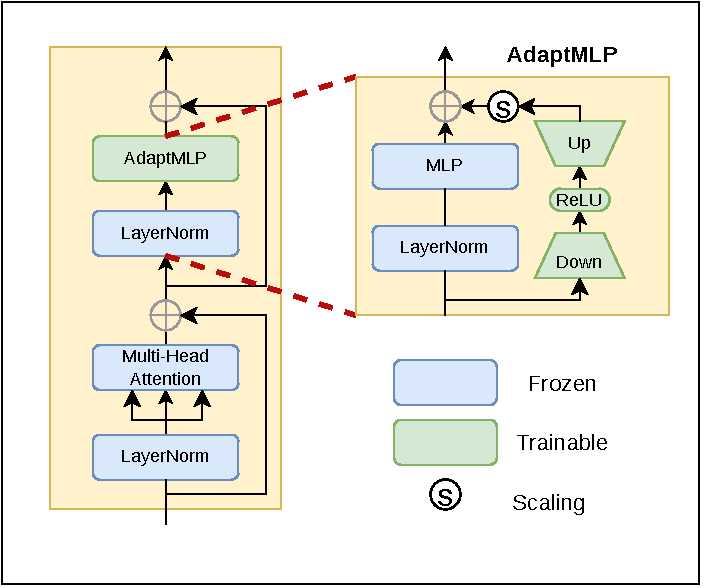
\includegraphics[width=0.8\textwidth]{images/adaptMLP.pdf}
        \caption{Architecture of the AdaptMLP module.}
        \label{fig:adapmlp}
    \end{figure}

    As illustrated in Figure~\ref{fig:adapmlp}, the adapter branch consists of three main components: a trainable down-projection layer, a ReLU activation function, and a trainable up-projection layer. The down-projection reduces the dimensionality of the input features, while the up-projection maps the resulting representation back to the original feature dimension.

    Let $d$ denote the feature dimension and $\hat{d}$ the bottleneck dimension, where $\hat{d} \ll d$. For a given input feature representation $x_0^l$, the adapter branch generates an adapted feature representation $\tilde{x}^l$, which can be expressed as:

    \[
    \tilde{x}^l =
    \operatorname{ReLU}\left(
    \operatorname{LN}(x_0^l) W_{\mathrm{down}}
    \right) W_{\mathrm{up}}.
    \]

    Here, $\operatorname{LN}$ denotes layer normalization, while $W_{\mathrm{down}}$ and $W_{\mathrm{up}}$ represent the trainable down-projection and up-projection weight matrices, respectively.

    Finally, the output of the original MLP branch and the adapted features are combined through residual connections with a scaling factor \(s\). The resulting output is given by:
    \[
        x^l = \operatorname{MLP}\left(\operatorname{LN}(x_0^l)\right)
        + s \cdot \tilde{x}^l + x_0^l.
        \]


    The first term represents the output of the original MLP, which retains the feature transformations learned during pretraining. The second term represents the adapted features produced by the lightweight adapter module, weighted by a scaling factor \(s\). This factor controls the influence of the adapter on the resulting feature representation. Finally, the original input \(x_0^l\) is added through a residual connection, preserving the input information and facilitating stable feature propagation. During fine-tuning, only the parameters of the adapter branch are updated, while the pretrained MLP and the remaining backbone parameters are kept frozen.

    % During the fine-tuning process, the pretrained Transformer backbone is kept frozen, and only the parameters of the adapter branch within the AdaptMLP module are updated. Specifically, the down-projection and up-projection layers are trainable, while the original MLP branch and the remaining backbone parameters remain unchanged. Since the adapter branch introduces only a small number of additional trainable parameters, task-specific adaptation could be achieved efficiently without modifying the majority of the pretrained model parameters.

    \subsection{Setup}

    To ensure a consistent adaptation strategy across vision models with different hidden dimensions, we adopt a fixed bottleneck reduction ratio of 12 rather than a fixed bottleneck dimension. Accordingly, the bottleneck dimension is determined proportionally to the hidden dimension of each backbone. This choice maintains a consistent relative adapter capacity across architectures while allowing the number of adapter parameters to scale with the size of the underlying model. Although AdaptFormer uses a bottleneck dimension of 64 in its default experimental configuration, this corresponds to a reduction factor of 12 for a ViT-Base model with a hidden dimension of 768. We therefore generalize the relative bottleneck configuration to the different vision backbones considered in this study.

    \section{Experimental Design}
\end{document}
